\documentclass{article}
\usepackage[margin=1.0in]{geometry}
\usepackage{amsmath}
\usepackage{float}
\usepackage{graphicx}
\usepackage{hyperref}


\title{Finance Club Project Application \\ \large 2022}
\author{
    \setlength{\tabcolsep}{12pt} % Default value: 6pt
    \renewcommand{\arraystretch}{2} % Default value: 1
    \begin{tabular}{|l|l|l|}
        \hline
        Name: Soham Roy                 & CGPA: 9.35     & Roll No: EE20B130      \\
        \hline
        Email Id: sroy@smail.iitm.ac.in & Hostel: Sindhu & Contact No: 9004077855 \\
        \hline
    \end{tabular}
}
\date{}
    
    
\begin{document}
\maketitle


\section*{Question 1}


\subsection*{a.}
The 4 option Greeks are a set of risk parameters regarding options, used to analyse the factors that influence option pricing. They are:

\begin{itemize}
    \item Delta ($\Delta$): The change in the option price with respect to a change in the underlying asset price.
          \begin{equation*}
              \Delta = \frac{\partial V}{\partial S},
          \end{equation*}
          \begin{center}
              where $V$ is the option price and $S$ is the underlying asset price.
          \end{center}
          If $S$ increases, the Call Option price increases, thus $\Delta > 0$ for Call options. \\
          If $S$ increases, the Put Option price decreases, thus $\Delta < 0$ for Put options. \\
          $\Delta$ can be interpreted as the probability of the option being profitable at expiration. \\
          $\Delta$ varies from -1 to 1, and $|\Delta| \approx 0.5$ for ATM (at-the-money) options. \\
          $|\Delta|$ is closer to 0 for OTM (out-of-the-money) options, and nearer to 1 for ITM (in-the-money) options.
          \begin{figure}[H]
              \centering
              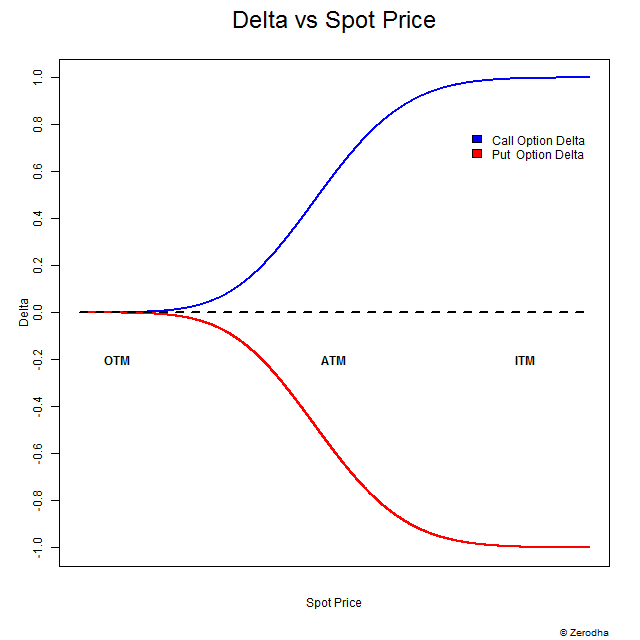
\includegraphics[scale=0.4]{Delta.png}
          \end{figure}

    \item Gamma ($\Gamma$): The change in the option Greek Delta with regards to the underlying asset price.
          \begin{equation*}
              \Gamma = \frac{\partial \Delta}{\partial S} = \frac{\partial^2 V}{\partial S^2},
          \end{equation*}
          \begin{center}
              where $\Delta$ is the option Greek Delta, $V$ is the option price and $S$ is the underlying asset price.
          \end{center}
          As $\Delta$ always increases with increase in $S$ and $|\Delta| < 1$, $\Gamma$ varies from 0 to 1. \\
          When the option is deep ITM or OTM, $|\Delta|$ saturates to 1, so its derivative $\Gamma$ tends to 0. \\
          Thus, $\Gamma$ is maximum when the option is ATM or nearly ATM. \\
          A low $\Gamma$ would imply that $\Delta$ is relatively stable and does not vary much with changes in $S$. \\
          A high $\Gamma$ would imply that $\Delta$ is relatively unstable and, thus, unpredictable and less reliable.
          \begin{figure}[H]
              \centering
              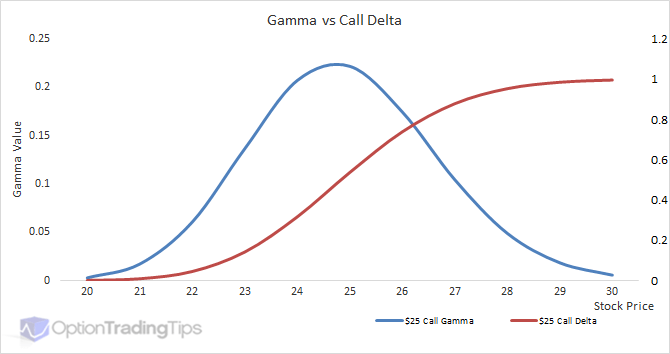
\includegraphics[scale=0.5]{Gamma.png}
          \end{figure}

    \item Theta ($\Theta$): The decrease in the option price resulting from a decrease in the time to maturity.
          \begin{equation*}
              \Theta = -\frac{\partial V}{\partial \tau},
          \end{equation*}
          \begin{center}
              where $V$ is the option price and $\tau$ is the time to maturity.
          \end{center}
          Options depreciate as their outcome becomes easier to predict with time to maturity approaching 0. \\
          $\Theta$ is a measure of the rate of this depreciation over time,  usually expressed as a negative number. \\
          ATM options are highly priced initially, and then depreciate fast ($|\Theta|$ increases) close to expiration. \\
          For deep ITM and OTM options, $|\Theta|$ is large initially and decreases when close to expiration.
          \begin{figure}[H]
              \centering
              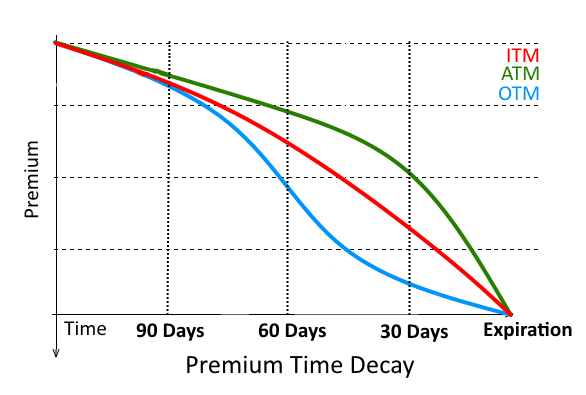
\includegraphics[scale=0.5]{Theta.png}
          \end{figure}

    \item Vega ($\mathcal{V}$): The change in the option price due to a change in the volatility of the underlying asset.
          \begin{equation*}
              \mathcal{V} = \frac{\partial V}{\partial \sigma},
          \end{equation*}
          \begin{center}
              where $V$ is the option price and $\sigma$ is the volatility of the underlying asset.
          \end{center}
          A high $\mathcal{V}$ implies that the option is more sensitive to changes in implied volatility. \\
          A high $\mathcal{V}$ is beneficial for option buyers, as it implies that the option might be profitable at some point. \\
          The converse is true for option sellers, who would want the option to expire unexercised. \\
          $\mathcal{V}$ is the highest for ATM options, declines as the option approaches expiration, and $\mathcal{V} > 0$ always.
          \begin{figure}[H]
            \centering
            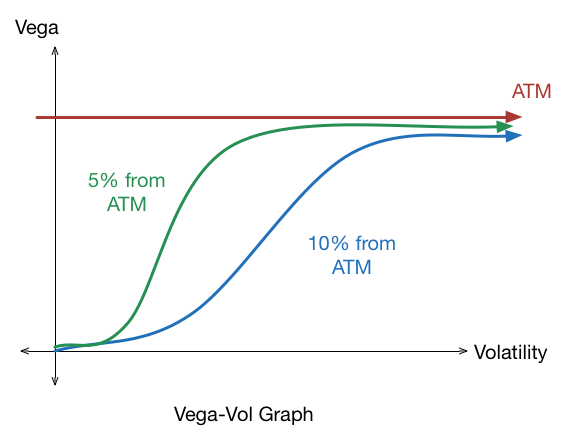
\includegraphics[scale=0.5]{Vega.png}
        \end{figure}
\end{itemize}


\subsection*{b.}

\subsubsection*{i.}
To make money if stock stays near the price when the orders were executed or goes below the price when the option was bought, we should: \\
\textbf{Sell Call Options}, \\
as the option would never be exercised if the stock goes below the original price. \\
Otherwise, we can assume that the stock stays near the original price, \\
implying that the increase in price would be less than the option's premium.

\subsubsection*{ii.}
To make money if volatility in the markets increases after executing the orders, we should: \\
\textbf{Buy Call Options} and \textbf{Buy Put Options}, \\
as we can expect the stock price to undergo either a large increase (i.e. profitable for our Call) \\
or a large decrease (i.e. profitable for our Put) if the volatility in the market increases. \\
As long as the volatility increases sufficiently, the large swing in the stock price will result in \\
the profit from either one or both of our Call or Put Options being much greater than the options' premiums.


\section*{Question 2}
\texttt{FinanceClub\_Project\_2022\_Soham\_EE20B130.ipynb} file attached with e-mail.


\section*{Question 3}
As mentioned in my resume at \href{http://sohamroy.ml/resume/}{sohamroy.ml/resume}, I have significant prior experience in coding. \\
\\
In addition to participating in competitive coding and other events / hackathons related to programming, \\
I have also worked on a number of projects. \\
They range from solving a Mouse Maze in C++ to implementing an OS in assembly and C, \\
and from interfacing a Discord bot in Python API to building websites in HTML/CSS/JS. \\
\\
I also worked under two CFI teams in the field of Deep Learning using Python, \\
and am presently working for Logistics Lab to implement novel algorithms for multi-drop container loading. \\
\\
I do not have any prior experience in finance, but I have always held an interest in it, \\
and I am always on the lookout for interesting opportunities, as evidenced by my varied prior experiences in coding.


\end{document}
